
\section{Implementation}
\label{Implementation}

In diesem Kapitel wird die Implementation der einzelnen Container beschrieben, wie sie im Kapitel \ref{Architektur:Container} definiert wurden.

\subsection{ÖV-Güteklassen 2018 Generator}
\label{Implementation:ÖV-Güteklassen 2018 Generator}

\subsubsection{Datenaufbereitung}
\label{ÖV-Güteklassen 2018 Generator:Datenaufbereitung}

Der \acs{ÖV}-Güteklassen 2018 Generator operiert auf unterschiedlichen Daten von externen Datenquellen.
Diese Daten kommen in den verschiedensten Formaten daher und müssen für eine weitere Verarbeitung gefiltert, aufbereitet und optimiert werden.
Für eine einfache Handhabung wurde ein Docker-Setup gewählt.
Die Bedienung dieses Setups ist im Kapitel \ref{Softwaredokumentation} ausführlich beschrieben.

Grundsätzlich kann man sagen, dass zwei Docker-Container existieren, namentlich \emph{tooling} und \emph{db}.
Der Docker-Container \emph{tooling} nimmt Daten in gängigen Formaten entgegen oder bezieht diese von externen Diensten und bereitet sie so vor, dass diese vom Docker-Container \emph{db} in die Datenbank \emph{oevgk18} für eine Weitereverwendung des \acs{ÖV}-Güteklassen 2018 Generator geladen werden können.
Der Docker-Container \emph{db} sorgt ebenfalls dafür, dass beim Starten die nötigen Extensions (pgrouting, hstore, \dots) aktiviert sind und zuerst die Schemas und danach die Stored Procedures erstellt werden.
Zusätzlich müssen nach den einzelnen Imports, welche nachfolgend beschrieben werden, zusätzliche Modifaktionen am Schema vorgenommen werden.
Diese Modifikationen werden in einem Post-Import-Schritt durchgeführt, weil die Terrain- sowie die OSM-Daten durch Tools importiert werden, welche ein Schema vorgeben und somit ein bereits modifiziertes Schema überschrieben wird. Ebenfall werden zusätzliche Indizes erstellt.

Im weiteren sind die Services, welche die beiden Docker-Container bereitstellen, anhand eines Datenflussdiagrams aufgeschlüsselt.
Der \acs{ÖV}-Güteklassen 2018 Generator operiert grundsätzlich auf drei externen Datenquellen, namentlich sind dass die Fahrplandaten (nachfolgend \emph{gtfs data}), das Terrainmodell (nachfolgend \emph{terrain data)} und die \acs{OSM}-Daten (nachfolgend \emph{osm data}).
Für jede Datenquelle existiert ein Service im Docker-Container \emph{tooling} und ein Pendant im Docker-Container \emph{db}, welche die vorverarbeiteten Daten des Docker-Container \emph{tooling} entgegennimmt und in die Datenbank spielt.

\paragraph{OSM-Daten}~\\
\acs{OSM}-Daten werden von der Routing-Enginge für das Berechnen von Isolinien und für das Identifizieren von \acs{ÖV}-Haltestellen verwendet.
In Abbildung \ref{fig:dataflow-docker-setup-osm-data} ist ersichtlich, wie der Docker-Container \emph{tooling} die \acs{PBF}-Datei der Schweiz von einem externen Dienst~\cite{planet_osm_ch} bezieht und für die zwei vorhin erwähnten Zwecke verarbeitet.

\begin{figure}[ht]
    \centering
    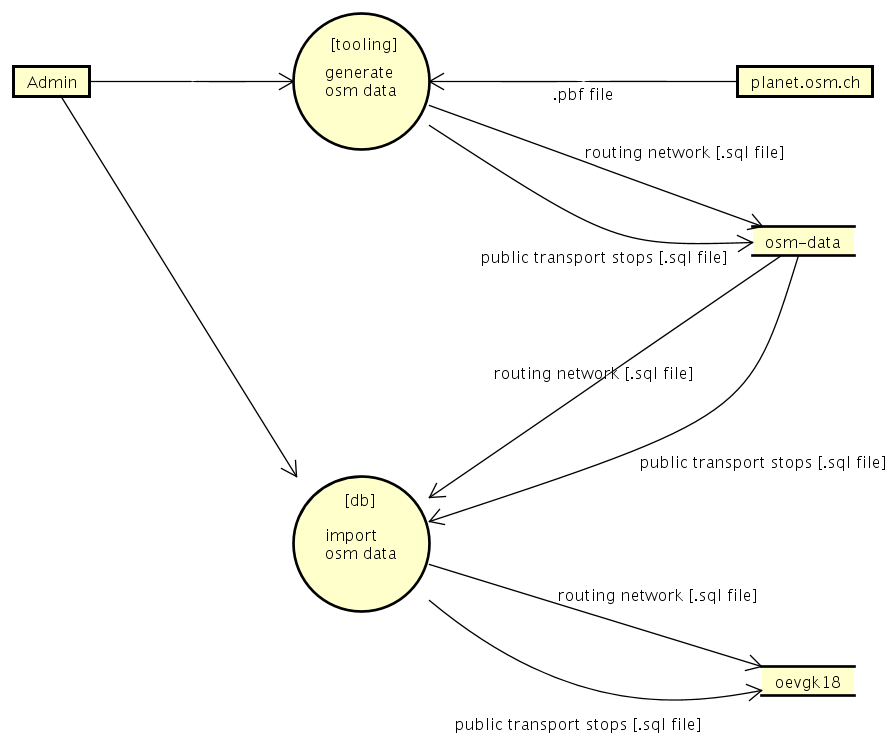
\includegraphics[width=0.8\linewidth]{projectdoc/img/dataflow-docker-setup-osm-data.png}
    \caption[Datenfluss Setup OSM-Daten]{Datenfluss Setup OSM-Daten}
    \label{fig:dataflow-docker-setup-osm-data}
\end{figure}

Das Routing-Netzwerk wird mithilfe des Tools \emph{OSM2PO}~\cite{OSM2PO} für pgrouting aufbereitet und als SQL-Datei bereitgestellt.
Die \acs{ÖV}-Haltestellen werden durch Osmosis~\cite{osmosis} gefiltert und ebenfalls in eine SQL-Datei exportiert.
Beide Tools werden durch separate Konfigurationen für unsere Zwecke konfiguriert.
So werden aus den \acs{OSM}-Daten für das Identifizieren von \acs{ÖV}-Haltestellen nur Nodes extrahiert, welche eine \emph{uic\_ref} besitzen. \ac{UIC}-Referenzen werden für die Identifizierung von \acs{ÖV}-Haltestellen verwendet.

\paragraph{GTFS-Daten}~\\
Die Fahrplandaten werden im Docker-Container \emph{tooling} automatisch von geOps~\ref{geops_fahrplandaten} im GTFS-Format~\cite{gtfs_spec} heruntergeladen und im CSV-Format als TXT-Dateien bereitgestellt.
Diese wiederum können in einem nächsten Schritt durch den Docker-Container \emph{db} in die Datenbank gespielt werden.
Der Datenfluss ist in Abbildung \ref{fig:dataflow-docker-setup-gtfs-data} ersichtlich.

\begin{figure}[ht]
    \centering
    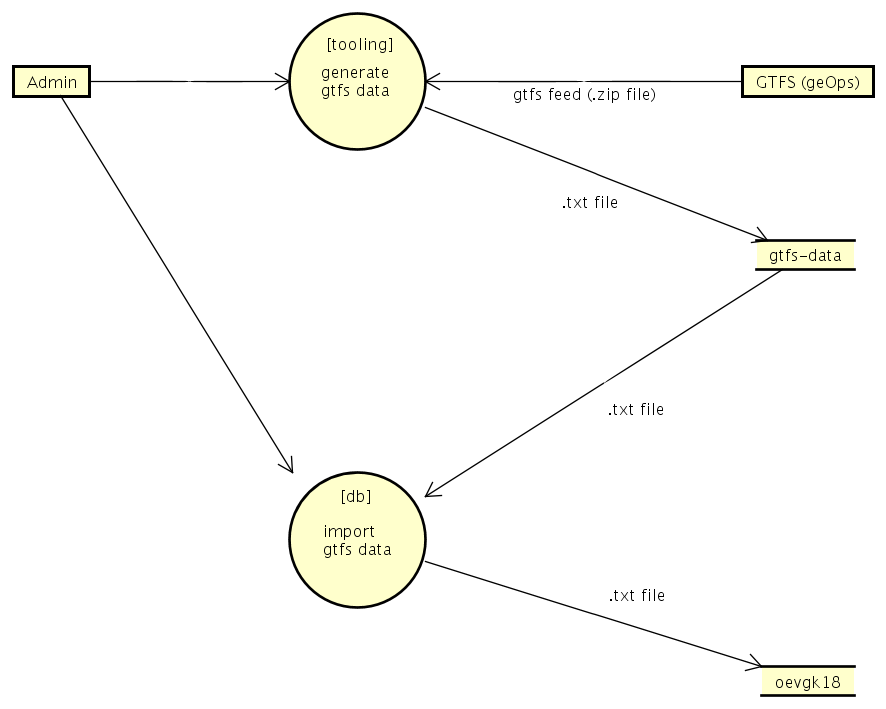
\includegraphics[width=0.8\linewidth]{projectdoc/img/dataflow-docker-setup-gtfs-data.png}
    \caption[Datenfluss Setup GTFS-Daten]{Datenfluss Setup GTFS-Daten}
    \label{fig:dataflow-docker-setup-gtfs-data}
\end{figure}

\paragraph{Terrain-Daten}~\\
Das Terrainmodell kann aufgrund der Grösse der Datei und aus lizenztechnischen Gründen nicht von einem externen Dienst bezogen und muss somit dem Service manuell als TIF-Datei bereitgestellt werden.
Diese Datei wird mit raster2pgsql~\cite{raster2pgsql}, einem Tool von PostGIS, welches Raster-Formate in ein Format konvertiert, welche in eine PostGIS-Tabelle geladen werden kann, verarbeitet.
Dabei wird von der üblichen Struktur (ein Service im Docker-Container \emph{tooling} und ein Pendant im \emph{db}) abgewichen.
raster2pgsql ist darauf ausgelegt direkt in eine PostgreSQL-Datenbank zu schreiben.
Der Weg über eine Intermediate-Datei wäre somit eine nicht begründete Indirektion.
Somit entfällt hier der Service im Docker-Container \emph{tooling}.
Der Datenfluss ist in Abbildung \ref{fig:dataflow-docker-setup-terrain-data} ersichtlich.

\begin{figure}[ht]
    \centering
    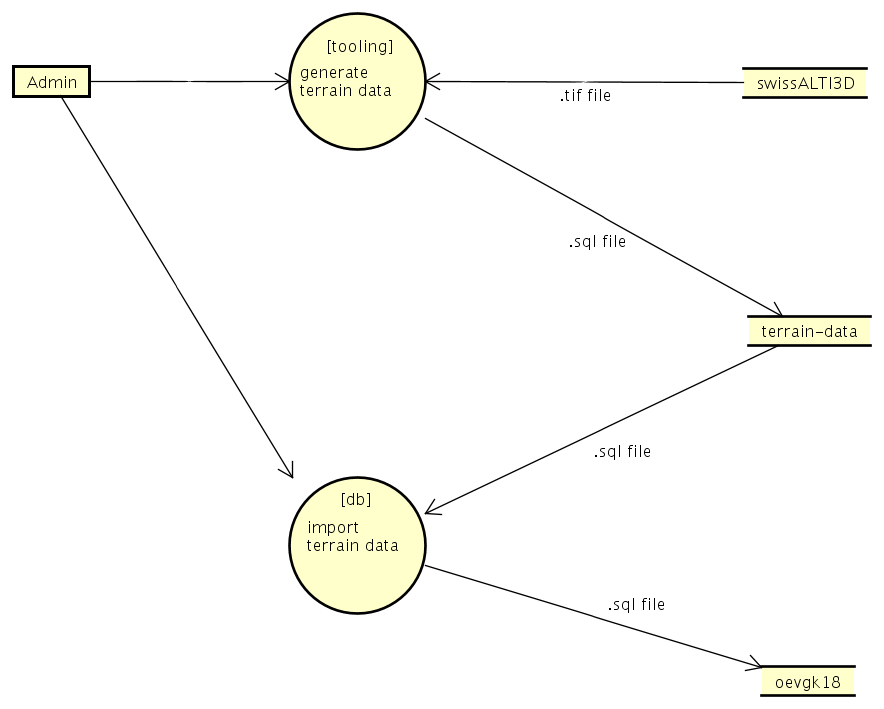
\includegraphics[width=0.8\linewidth]{projectdoc/img/dataflow-docker-setup-terrain-data.png}
    \caption[Datenfluss Setup Terrain-Daten]{Datenfluss Setup Terrain-Daten}
    \label{fig:dataflow-docker-setup-terrain-data}
\end{figure}

\subsubsection{Umsetzung Spezifikation}
\label{ÖV-Güteklassen 2018 Generator:Umsetzung Spezifikation}

\paragraph{Datenfluss}~\\
Durch die unterschiedliche Natur der Datenquellen und der Menge dieser ist es hilfreich, zu visualisieren, zu welchem Zeitpunkt, welche Daten zu welchen Zweck benötigt werden.
Wie in Abbildung \ref{fig:Flow_OeVGK_Brechnung} ersichtlich ist, werden die \acs{ÖV}-Güteklassen in fünf Schritten berechnet. 
In Abbildung \ref{fig:dataflow_OeV-Gueteklassen_2018_Generator} ist nun schematisch die Raison d’Être der Datenquellen ersichtlich.

\begin{figure}[ht]
    \centering
    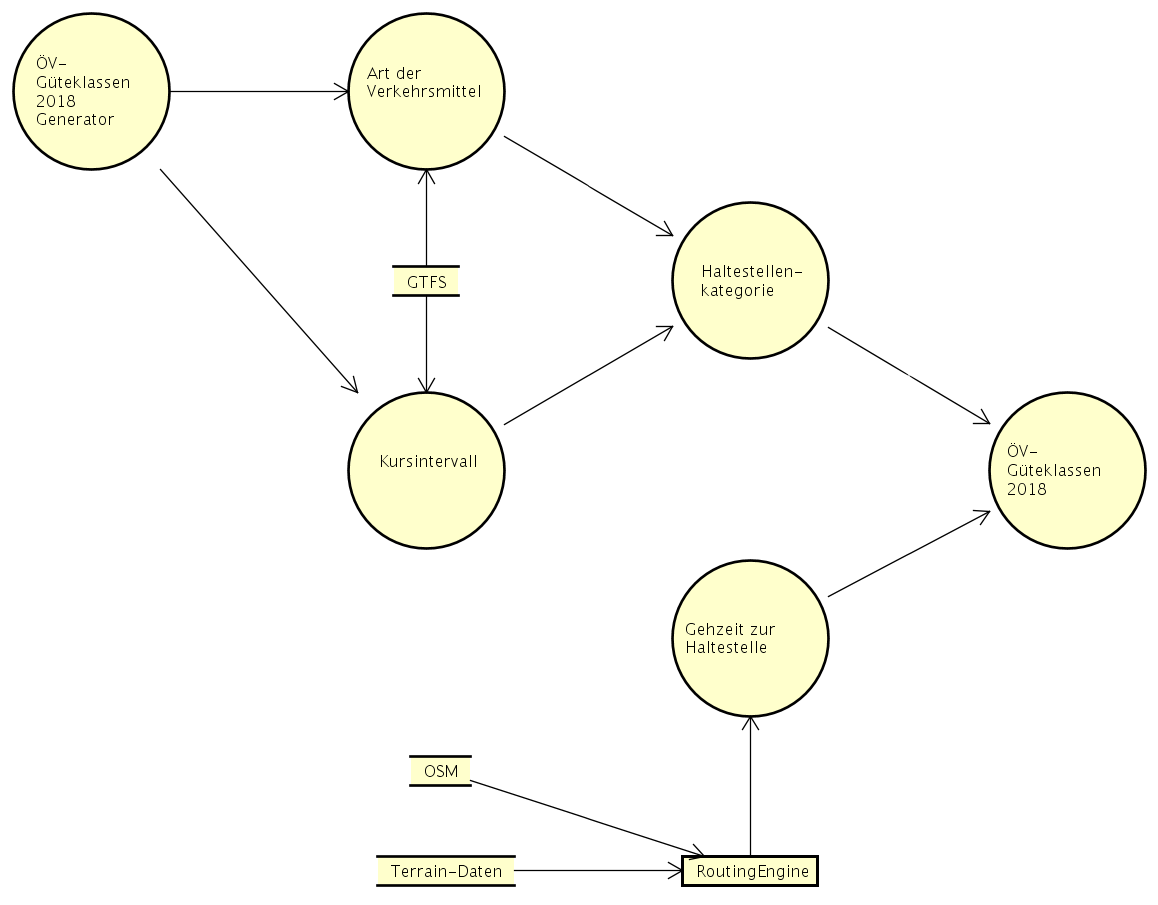
\includegraphics[width=1.0\linewidth]{projectdoc/img/dataflow_OeV-Gueteklassen_2018_Generator.png}
    \caption[Datenfluss ÖV-Güteklassen 2018 Generator]{Datenfluss ÖV-Güteklassen 2018 Generator}
    \label{fig:dataflow_OeV-Gueteklassen_2018_Generator}
\end{figure}

Die Datenquellen \emph{GTFS}, \emph{OSM} und \emph{Terrain-Daten} entsprechen an sich keinen separaten Datenquellen, sondern werden nur zum besseren Verständnis getrennt dargestellt.
Wie wir in Kapitel \ref{ÖV-Güteklassen 2018 Generator:Datenaufbereitung} gesehen haben, werden diese aufbereitet und optimiert in einer Datenbank \emph{oevgk18} gehalten.

Nachfolgend werden die fünf Berechnungsschritte separat beschrieben.

\paragraph{Berechnung der Art der Verkehsmittel}~\\
Die öffentlichen Verkehrsmittel werden in drei Verkehrsmittelgruppen gruppiert (siehe Kapitel \ref{Berechnungsmethodik OeVGK18:Art der Verkehrsmittel}).
Wie in Kapitel \ref{subsystem:GTFS} beschrieben, werden die Fahrplandaten im \acs{GTFS}-Format~\cite{gtfs_spec} gehalten. 
Es werden dabei 8 Verkehrsmittel-Typen unterschieden.
In Tabelle \ref{table:Mapping GTFS Route Type Verkehrsmittelgruppe} ist ein Mapping der definierten GTFS Route Typen und der Verkehrsmittelgruppen ersichtlich.

\begin{table}[ht]
    \centering
    \begin{tabular}[ht]{l l}
        \toprule
        \textbf{GTFS Route Type} 
                                & \textbf{Verkehrsmittelgruppe}\\
        \midrule
        0 (Tram, Streetcar, Light rail)
                                & C\\
        1 (Subway, Metro)
                                & A/B\\
        2 (Rail)
                                & A/B\\
        3 (Bus)
                                & C\\
        4 (Ferry)
                                & C\\
        5 (Cable car)
                                & C\\
        6 (Gondola, Suspended cable car)
                                & C\\
        7 (Funicular)
                                & C\\            
        \bottomrule
    \end{tabular}
    \caption{Mapping GTFS Route Type Verkehrsmittelgruppe}
    \label{table:Mapping GTFS Route Type Verkehrsmittelgruppe}
\end{table}

Die Herausforderung beim Berechnen der Art der Verkehrsmittel ist die Evaluation der Bahnknoten.
Die Definition des Bahnknoten ist im Kapitel \ref{Berechnungsmethodik OeVGK18:Art der Verkehrsmittel} genau spezifiziert.
Für die Klassifizierung eines Bahnknoten ist die Anzahl der Richtungen, in welche man von einer Bahnstation aus verkehren kann, relevant.

\begin{listing}[ht]
    \inputminted{sql}{projectdoc/listing/count_of_distinct_next_stops.sql}
    \caption{SQL-Query zur Bestimmung der Anzahl erreichbaren Haltestellen}
    \label{listing:count_of_distinct_next_stops}
\end{listing}

In Listing \ref{listing:count_of_distinct_next_stops} ist ersichtlich, wie für eine spezifizierte Auswahl an Haltestellen (\emph{relevant\_stops}) die Anzahl erreichbaren Haltestellen gezählt wird.
Im abgebildeten Query wird geprüft, ob der aktuelle Stop bei einem anderen \emph{Trip} als vorherige Haltestelle vorkommt.
Die Anzahl wird mit der Window Function gesammelt und gruppiert für jede Haltestelle retourniert.

Die abgebildete Berechnung hat mehrere Verbesserungen und Ver­schlimm­bes­se­rungen durchlaufen.
Es lohnt sich einen ausführlicheren Blick auf die Evolution der Abfragetechnik zu legen, da diese Hoch und Tiefs durchlebt hat und einige Learnings daraus gezogen wurden.

\subparagraph{1. Version}
In einer ersten Version war angedacht, dass das Berechnen der Anzahl erreichbaren Haltestelle für jede einzelne Haltestelle separat aufgerufen wird.

\begin{listing}[ht]
    \inputminted{sql}{projectdoc/listing/count_of_distinct_next_stops_v1.sql}
    \caption{SQL-Query zur Bestimmung der Anzahl erreichbaren Haltestellen (Version 1)}
    \label{listing:count_of_distinct_next_stops_v1}
\end{listing}

Das Datenmodell von GTFS zwingt einem zu einem Join über mehrere grössere Tabelle, welcher mehrmals durchgeführt werden muss.
In Listing \ref{listing:count_of_distinct_next_stops_v1} ist ersichtlich, wie in einer Common Table Expression dieser für jede Haltestelle durchgeführt wird.
Dieser Join bildet für eine Station alle \emph{Trips} mit der Nummer des akutellen \emph{Stops} auf einem \emph{Trip} ab.
Dieser Join ist sehr zeit- und ressourcenintensiv.
Diese Abfrage dauert pro Haltestelle 11.9 Sekunden, was bei momentan akuellen 1815 Bahnhaltestellen extrem ins Gewicht fällt.

\subparagraph{2. Version}
In einer zweiten Version war die Überlegung den Join zu persistieren, damit nicht jede Abfrage diese aufwändigen Join durchführen muss und Indizes darauf zu generieren.

Der Grund warum in diesem Fall nicht eine temporäre Tabelle in Frage kommt, ist in der PostgreSQL-Dokumentation beschrieben: "`The autovacuum daemon cannot access and therefore cannot vacuum or analyze temporary tables."'~\cite{postgresql_doc}
Es ist auch nicht möglich den Daemon manuell anzustossen, da das Erstellen der temporären Tabelle und das Starten des Daemons aus einer PostgreSQL-Funktion nicht in der selben Session durchgeführt werden kann, was den Nutzen der temporären Tabelle zu nichte macht, denn damit die Indizes greifen, ist dieser Prozess relevant.
Das Persistieren des Join und das Anlegen der Indizes bringen in diesem Fall eine enorme Performanzsteigerung, wie in Tabelle \ref{table:Performanzvergleich Temp Table und Table mit Index} ersichtlich ist, mit der Annahme, dass Autovacuum lief.

\begin{table}[ht]
    \centering
    \begin{tabular}[ht]{l l l}
        \toprule
        \textbf{} 
                                & \textbf{temporäre Tabelle}
                                & \textbf{Tabelle}\\
        \midrule
        Erstellen der Tabelle
                                & 6.7 s
                                & 7.3 s\\
        Erstellen der Indizes
                                & -
                                & 3.9 s\\
        Abfrage
                                & n * 4.8 s
                                & n * 0.062 s\\        
        \bottomrule
    \end{tabular}
    \caption{Performanzvergleich Temp Table und Table mit Index}
    \label{table:Performanzvergleich Temp Table und Table mit Index}
\end{table}

\subparagraph{3. Version}
Um die Datenbank nicht mit fast 2000 Abfragen für alle Bahnhaltestellen zu belasten, entstand die Idee für alle Haltestellen in einer Abfrage die erreichbaren Haltestellen zu zählen.

\begin{listing}[ht]
    \inputminted{sql}{projectdoc/listing/count_of_distinct_next_stops_v3.sql}
    \caption{SQL-Query zur Bestimmung der Anzahl erreichbaren Haltestellen (Version 3)}
    \label{listing:count_of_distinct_next_stops_v3}
\end{listing}

Dazu wurde die Abfrage in die Version, welche in Listing \ref{listing:count_of_distinct_next_stops_v3} ersichtlich ist umgebaut.
Die Abfrage läuft in 9.8 Sekunden und ist im Vergleich zur Lösung aus Version 2 für momentan 1815 vorhandenen Bahnhaltestellen um über 100 Sekunden schneller.

\subparagraph{Finale Version}
Da nun die Berechnung nicht mehr für alle Bahnhaltestellen einzeln durchgeführt wird, lohnt sich die Analyse, ob sich die Erstellung der Tabelle (\emph{next\_station\_mapping}) und der Indizes im Vergleich zum Join in einer Common Table Expression noch lohnt.

\begin{table}[ht]
    \centering
    \begin{tabular}[ht]{l l l}
        \toprule
        \textbf{} 
                                & \textbf{Join in Tabelle}
                                & \textbf{Join in CTE}\\
        \midrule
        Erstellen der Tabelle
                                & 7.3 s
                                & - \\
        Erstellen der Indizes
                                & 3.9 s
                                & - \\
        Abfrage
                                & 9.8 s
                                & n * 0.062 s\\
        \textbf{Total}
                                & \textbf{21 s}
                                & \textbf{17.5 s}\\            
        \bottomrule
    \end{tabular}
    \caption{Performanzvergleich Join in Tabelle und Join in CTE}
    \label{table:Performanzvergleich Join in Tabelle und Join in CTE}
\end{table}

In der Tabelle \ref{table:Performanzvergleich Join in Tabelle und Join in CTE} ist das Ergebnis ersichtlich.
Die Performanzverbesserung ist durch die Natur des OeVGK18-Generator ein Tropfen auf dem heissen Stein, jedoch wird die Verbesserung übernommen, da in dieser Variante nicht zusätzliche eine Tabelle angelegt werden muss, welche nur für einen Join benötigt wird und sonst nichts mit der Domain zu tun hat.

Die finale Version war bereits in Listing \ref{listing:count_of_distinct_next_stops} ersichtlich.

\subparagraph{Fazit}
Optimierungen, welche in der 2. und 3. Version Sinn gemacht haben, war in der finalen Version dann nicht mehr notwendig.
Es hat sich gezeigt, dass es sich lohnt, vergangene Annahmen zu überdenken und zu prüfen, ob diese auf die aktuelle Situation immer noch zu treffen.
In Tabelle \ref{table:Performanzvergleich der verschiedenen Version} sind die Resultate der Optimierungen zusammengefasst.

\begin{table}[ht]
    \centering
    \begin{tabular}[ht]{l l}
        \toprule
        \textbf{Version} 
                                & \textbf{Dauer}\\
        \midrule
        Version 1
                                & 360 min\\
        Version 2
                                & 112.53 s\\
        Version 3
                                & 21 s\\
        \textbf{Finale Version}
                                & \textbf{17.5 s}\\            
        \bottomrule
    \end{tabular}
    \caption{Performanzvergleich der verschiedenen Version}
    \label{table:Performanzvergleich der verschiedenen Version}
\end{table}

\paragraph{Berechnung des Kursintervalls}~\\
Für die Berechnung des Kursintervalls wurde die Formel, wie sie in der Spezifikation (siehe Kapitel \ref{Berechnungsmethodik OeVGK18:Kursintervall}) definiert wurde, direkt umgesetzt.
Um alle Abfahrtszeiten einer Haltestelle zu erhalten, wurde zuerst eine SQL-Query für die GTFS-Datenbank formuliert, in der nach der \acs{UIC}-Referenz gefiltert wird.
Die Ausführung dieser Query dauerte allerdings ca. 1.7 Sekunden pro Haltestelle, was bei einer Gesamtzahl von 28'000 Haltestellen etwa 11 Stunden dauern würde.

Viel effizienter ist es, die Abfahrtszeiten für alle Haltestellen in einer einzelnen Abfrage zu aggregieren.
Diese ist in Listing \ref{listing:sql_query_departure_times} abgebildet.
Die optimierte SQL-Query dauert ca. 7 Sekunden für alle 28'000 Haltestellen, was eine drastische Verbesserung darstellt.

\begin{listing}[ht]
    \inputminted{sql}{projectdoc/listing/departure_time_cte.sql}
    \caption{Effiziente SQL-Query zur Abfrage aller Abfahrtszeiten an einem bestimmten Tag}
    \label{listing:sql_query_departure_times}
\end{listing}

\paragraph{Berechnung der Haltestellenkategorie}~\\
TODO

\paragraph{Berechnung der Gehzeit zur Haltestelle}~\\

\subparagraph{Snapping von der Haltestelle auf den Routing-Graph}
Die Haltestellen stammen aus dem Datenstamm der SBB~\cite{sbb_hafas_spec} und sind somit nicht Teil des Routing-Graphen. 
Um die \glspl{Isochrone} berechnen zu können, muss auf dem Routing-Graphen zuerst ein Startpunkt ermittelt werden, von dem das Routing entlang der Strassen und Wege ausgehen kann.
Dieser Punkt soll möglichst nahe an der eigentlichen Haltestelle liegen.
Es ist anzumerken, dass unsere Fahrplan-Daten lediglich ein geographischer Punkt pro Haltestelle definiert und so Buskanten oder Gleise nicht genau abbilden.

Ein erster Ansatz dieses "`Snappings"' sucht den geographisch nächstliegenden Vertex des Routing-Graphen zu den Koordinaten der Haltestelle.
Dies ist bei regulären Bushaltestellen mit zwei Kanten ein guter Ansatz, da diese Koordinaten meist neben oder direkt auf der Strasse liegen.
Problematisch wird dies aber etwa bei grossen Bahnhöfen wie dem Zürcher Hauptbahnhof.
Die Koordinate des Bahnhofs liegt in der Mitte der Bahnhofshalle, welche als Fussgängerfläche erfasst ist.
Da solche Flächen nicht im Routing-Graphen abgebildet werden, liegt der nächste Vertex des Routing-Graphen auf einer Rolltreppe, die nicht mit dem restlichen Graphen verbunden ist (siehe Abbildung~\ref{fig:snapping_comparison}).
Dieses Snapping auf einen isolierten Graphen führt dazu, dass die Routing-Engine nie ausserhalb des Bahnhofs routen kann, dadurch können auch keine \glspl{Isochrone} erzeugt werden.

\begin{figure}[ht]
    \centering
    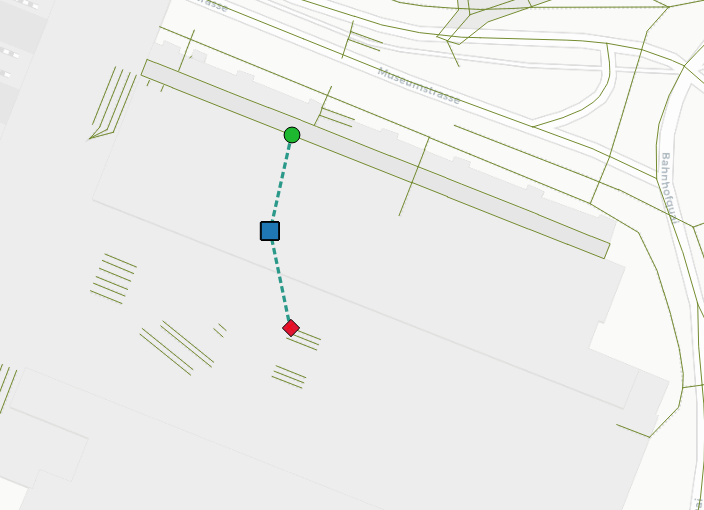
\includegraphics[width=1\linewidth]{projectdoc/img/snapping_comparison}
    \caption[Snapping der Haltestelle auf den Routing-Graphen]{Die Haltestelle (blaues Quadrat) wird mit dem einfachen Ansatz zur Rolltreppe `"gesnapped"' (Roter Diamant), während die Optimierung (Grüner Punkt) ein Ergebnis erzeugt, dass mit dem restlichen Routing-Netz verbunden ist.}
    \label{fig:snapping_comparison}
\end{figure}

Ein optimierter Ansatz nimmt nicht direkt den nächstgelegen Punkt auf dem Routing-Graphen, sondern prüft, ob der ermittelte Vertex auf einem isolierten Segment des Graphen liegt.
Dafür werden mit Hilfe der Routing-Engine alle Punkte gesucht, die auf dem Graphen in 200 Metern Fussweg erreichbar sind.
Wenn es einen Punkt gibt, der mindestens 150 Meter entfernt vom Startpunkt ist, wird dies als genügend bewertet, um den Startpunkt für die Erzeugung von \glspl{Isochrone} zu verwenden.
Wenn diese Bedingung nicht erfüllt ist, werden iterativ andere Vertices geprüft (sortiert nach der Distanz zur Haltestelle), bis ein passender Vertex gefunden wird.
Der Code dazu ist in Listing \ref{listing:snap_routing_graph} ersichtlich.

\begin{listing}[ht]
    \inputminted{sql}{projectdoc/listing/nearest_neighbor.sql}
    \caption{SQL Stored Procedure für das "`Snapping"' der Haltestelle auf den Routing-Graph}
    \label{listing:snap_routing_graph}
\end{listing}

Das Ergebnis für den Zürcher Hauptbahnhof ist in Abbildung~\ref{fig:snapping_comparison} zu sehen.
Dieser Startpunkt ist noch immer nicht optimal, da ein Fussgänger auch ein Ausgang auf der anderen Seite des Bahnhofes wählen könnte.
Für eine optimale Bestimmung müsste der Routing-Graph mit zusätzlichen Wegen ergänzt werden.
Fussgängerflächen könnten beispielsweise durch eine Vorverarbeitung durch \emph{PlazaRoute}~\cite{plaza_route} in den Routing-Graph integriert werden. Dabei werden zusätzliche Graph-Kanten eingefügt.


\paragraph{Berechnung der ÖV-Güteklassen}~\\
TODO 

